\section{Blatt}


\begin{aufg}[6 Punkte]
Romeo m\"ochte Julia besuchen, aber zwischen den beiden ist ein $9$ Meter breiter Fluss. Romeo hat beliebig viele Holzbalken der L\"ange~$1$~m (Breite ~$50$ cm, H\"ohe $10$~cm) zur Verf\"ugung, aus denen er versucht will, eine Br\"ucke von der Form wie im Bild unten (Abbildung~\ref{fig:romeo}) zu bauen. Weiterhin hat er ein beliebig langes Seil, das er am oberen Ende der Br\"ucke befestigen will, um sich herunterzulassen. Die Br\"ucke ist stabil, wenn f\"ur jeden benutzten Holzbalken gilt, dass der Schwerpunkt der Brückenkonstruktion auf diesem Holzbalken \"uber diesem Holzbalken liegt. Das Gewicht von Romeo und dem Seil d\"urfen wir vernachl\"assigen, ebenso die m\"oglichen Probleme bei der Anbringung des Seiles. Schafft Romeo es, zu Julia zu kommen? (Genaue Begr\"undung!)
%
\begin{figure}
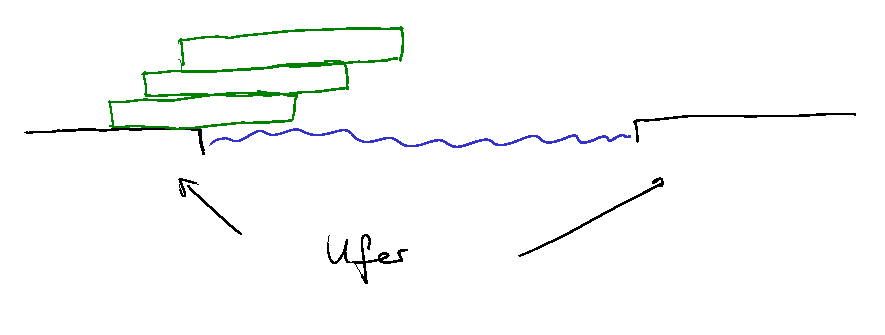
\includegraphics{romeo.pdf}
\caption{Romeos Br\"ucke}\label{fig:romeo} 
\end{figure}
%
\end{aufg}

\bigskip

\begin{lsg}
\end{lsg}


\bigskip


\begin{aufg}[6 Punkte]
Bestimmen Sie folgende Grenzwerte:
\begin{enumerate}[label=$\mathrm{(\roman*)}$, ref=$\mathrm{\roman*}$]
\setlength{\itemsep}{4pt}
\item $ \lim\limits_{x\to \infty} \dfrac{x^{2021}-17x^{10}}{x^{2022}+x+3} $,
\item $ \lim\limits_{x\to 2} \dfrac{x^{2}-3x+2}{x^{2}-x-2} $,
\item $ \lim\limits_{x\to 2} \left(1-\dfrac{2}{x}\right)^{2} \left( \dfrac{x^{7}-4x}{(x-2)^{2}} \right) $.
\end{enumerate}
\end{aufg}

\bigskip

\begin{lsg}\mbox{ }
\begin{enumerate}[label=$\mathrm{(\roman*)}$, ref=$\mathrm{\roman*}$]
\setlength{\itemsep}{4pt}
\item 
\end{enumerate}
\end{lsg}

\bigskip

\begin{aufg}[6 Punkte]
Die Exponentialfunktion $\exp\colon\R\to\R$ ist gegeben durch (siehe Vorlesung)
\[
\exp(x)\coloneqq \sum_{k=0}^{\infty}\frac{x^k}{k!}\,. 
\]
\begin{enumerate}[label=$\mathrm{(\roman*)}$, ref=$\mathrm{\roman*}$]
\item Zeigen Sie, dass $\exp(x)\cdot \exp(y)=\exp(x+y)$ \emph{(Hinweis: Cauchy-Produkt)}.
\item Zeigen Sie, dass die Exponentialfunktion auf ganz $\R$ stetig ist, d.h., f\"ur jedes~$x_0\in\R$ ist der Grenzwert von~$\exp$ in~$x_0$ gerade $\exp(x_0)$.
\end{enumerate}
\end{aufg}
 
\bigskip

\begin{lsg}\mbox{ }
\begin{enumerate}[label=$\mathrm{(\roman*)}$, ref=$\mathrm{\roman*}$]
\item 
\end{enumerate}
\end{lsg}

\bigskip


\begin{aufg}[6 Punkte]
Die \textit{Riemannsche Zeta-Funktion} wird definiert durch die Reihe 
\[
\zeta(s) = \sum_{k=1}^{\infty} \frac{1}{k^{s}}
\]
f\"ur alle $s\in \R$, $s>1$. Zeigen Sie, dass $\zeta(n) < 2$ f\"ur alle nat\"urlichen Zahlen $n\geq 2$. 

\noindent
\emph{Hinweis:} Betrachten Sie zuerst
\[
\sum_{n=2}^{\infty} \sum_{k=2}^{\infty} \frac{1}{k^{n}}\,.
\]
\end{aufg}


\bigskip

\begin{lsg}[Zehra Ciftci, Sude Cinar, Saveen Kassem]

Z.z.: $\zeta(n) < 2$ f\"ur alle nat\"urlichen Zahlen $n\geq 2$. 


Es gilt nach Beispiel 3.60: 

\[ \displaystyle\sum_{k=1}^{\infty}\frac{1}{k^{2}}\]

ist eine konvergente Majorante für

\[ \displaystyle\sum_{k=1}^{\infty}\frac{1}{k^{m}}\] 

mit natürlichem $m > 2$. Außerdem gilt: $k^m > k^2$  genau dann, wenn  
$$\frac{1}{k^2} < \frac{1}{k^m}$$.

Auch gilt, dass die erste Patrialsumme mit dem Wert 1 gleich ist.

In Übungsblatt 8 wurde bewiesen, dass 

\[ \displaystyle\sum_{k=1}^{\infty}\frac{2}{(k+1)}=2\]

eine konvergente Majorante für 

\[ \displaystyle\sum_{k=1}^{\infty}\frac{1}{k^{2}}\]

und dass das erste Glied der Reihe gleich ist.

Somit entspricht: 


\begin{align*}
 \displaystyle\sum_{k=1}^{\infty}\frac{1}{k^{2}} < 
\displaystyle\sum_{k=1}^{\infty}\frac{2}{(k+1)}=2.
\end{align*}

Nach dem Axiom der Transitivität der Anorndnung gilt: 
\begin{align*}
\displaystyle\sum_{k=1}^{\infty}\frac{1}{k^{m}} 
& < \displaystyle\sum_{k=1}^{\infty}\frac{1}{k^{2}}
\\
& < \displaystyle\sum_{k=1}^{\infty}\frac{2}{(k+1)}=2
\end{align*}

Nun kann man mit der Definition der Riemannschen-Zeta-Funktion ausdrücken, dass 
mit einer weiterhin natürlichen Zahl größer 2 folgendes gilt:
\begin{align*}
 \zeta(m) = \displaystyle\sum_{k=1}^{\infty}\frac{1}{k^{m}}
& <
\zeta(2) = \displaystyle\sum_{k=1}^{\infty}\frac{1}{k^{2}}
\\ 
& <
\displaystyle\sum_{k=1}^{\infty}\frac{2}{(k+1)}=2
\end{align*}

also kurz: $$ \zeta(m) < \zeta(2) < 2 $$.

Somit wurde $\zeta(n) < 2$ f\"ur alle nat\"urlichen Zahlen $n\geq 2$ gezeigt.
\end{lsg}
 
\bigskip

\begin{aufg}[2 Punkte; Sonderaufgabe]
Wenn Sie Aufgabe~8.5 abgegeben haben (womit Sie sich 2 Punkte verdient haben), erhalten Sie von ihrer \"Ubungsleiterin oder Ihrem \"Ubungsleiter die Abgabe einer anderen Gruppe. Korrigieren Sie diese Abgabe und bepunkten Sie sie. Sie haben 6 Punkte zur Verf\"ugung. (Die andere Gruppe erh\"alt nicht die Punkte, die Sie vergeben, sondern die 2 Punkte f\"ur das Abgeben.) Achten Sie beim Korrigieren insbesondere auf Folgendes: 
\begin{itemize}
 \item Alle Stellen, die falsch sind, anmerken und erkl\"aren, was falsch ist.
 \item Alle Stellen, die unverst\"andlich sind, anmerken und erkl\"aren, was unverst\"andlich ist.
\end{itemize}
Kurzum, Sie machen die Korrektur so, wie Sie erwarten, dass Ihre Abgaben korrigiert werden. Ihr Korrekturergebnis soll so sein, dass Sie hinterher erkl\"aren k\"onnen, was falsch und was richtig an der Abgabe ist. Sie geben die Korrektur dann mit Ihrer Abgabe von Blatt~9 am 21.12. in den \"Ubungsgruppen ab.
\end{aufg}

